\section{Background}
\label{sec:background}
This chapter will delve into the background of the project, exploring the existing literature on computer vision systems for component identification, real-time computer vision architectures, and the mechanical design of existing sorting machines. This research will inform the design of the project and its various systems. Research into these topics will inform the decisions made in the design of the project and its various systems.

\subsection{Existing Computer Vision Techniques}
A range of computer vision techniques have been explored in the literature, ranging from PCA (Principle Component Analysis) by \citet{Dhenge2013MechanicalNS} to more modern computer vision techniques like CNNs as used by \citet{Xu2020,s22239079}. However, given the rate of advancement of computer vision techniques, the techniques used in the literature reflect the state of the art at the time of writing, and so are not necessarily the most viable current techniques for the project, but they inspire novel approaches to the problem of component identification.

PCA with ANN (Artificial Neural Networks) as used by \citet{Dhenge2013MechanicalNS} is a relatively simple but outdated statistical technique that was successful in identifying nuts and bolts, which are very distinct components. In this paper, PCA is used as a feature extractor and then fed directly into, though not explicitly mentioned, an FCL (Fully Connected Layer), as the classifier. Although a valid approach, CNNs (Convolutional Neural Networks) are known to be much more effective at feature extraction, and do not "have the problem of low recall and accuracy", as mentioned by \citet{Xu2020}, that PCA may suffer from, so this approach may not be the most viable for the project. PCA excels at identifying components that are very distinct, like nuts and bolts, but may struggle with components that are more similar, like different types of capacitors, which is a problem that the project may face. To support this claim, \citet{Xu2020} use the SqueezeNet CNN architecture to identify 22 different subcategories of electronic components, specifically resistors, capacitors, and inductors, which is directly applicable to the project. They achieve a TPR (True Positive Rate) of 99.999\% with only a 2.67ms average inference time on a GTX 1050 2GB GPU (released in 2016), which would translate to ~374 FPS (Frames Per Second); a very impressive result. This work helps to support the claim that a CNN is a more viable approach to the problem of component identification, and so this will inform the design of the project's computer vision system.

\begin{figure}[H]
  \hfill
  \begin{minipage}[t]{\textwidth}
    \centering
    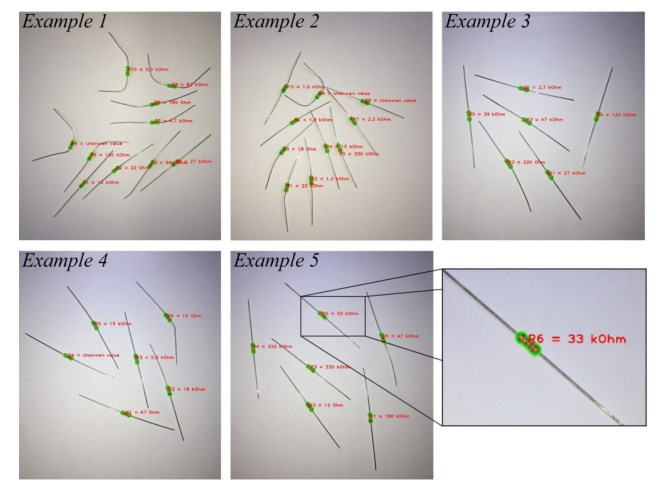
\includegraphics[height=8cm]{imgs/articles/resistordata.jpg}
    \caption{Resistor Test Set \cite{8939034}}
    \label{fig:resistordata}
  \end{minipage}
\end{figure}

The paper by \citet{8939034} discusses the use of an SVM (Support Vector Machine) to characterise resistors, by identifying the resistor's centroid (centre of mass), determining the resistor's orientation, and then analysing the bands to determine the resistor's value. This is directly applicable to the project, as it is a viable approach to identifying resistors, which are very distinct from other components, given the presence of colour bands. The paper's novel approach to identifying the resistor values allows it to achieve high accuracy of 86\%. However, this is calculated on a per-resistor basis --- an incorrect band does not mean the entire resistor is incorrect, which is not the case in the project's vision system, where the entire component must be identified correctly otherwise it will be sorted incorrectly. The images are also taken from a distance as shown in \autoref{fig:resistordata}, which may make the bands appear smaller than they would in the project's vision system, which may affect the accuracy of the approach.

The inference time seems to be incredibly fast, only being ~0.7ms, although it is important to note this was run on an Intel® Core™ i5-6200U CPU, rather than an edge device like the Raspberry Pi 4, which may have a slower inference time. In any case, it shows that the SVM is a viable approach to consider for the project.

\subsection{Computer Vision Architectures}
\label{sec:background-computer-vision}
For the problem of component identification, the computer vision system must be able to identify components in real-time, as the components may eventually be moving on a conveyor belt, captured using a camera facing down at the components. This means that the computer vision system must be able to identify components in a very short amount of time, or in other words, have a short inference time, and so the system must be computationally efficient. The envisioned system is designed to be self-contained, and as described in \autoref{sec:design-and-system-architecture}, the system will run on a Raspberry Pi 4, which has a 1.8GHz quad-core 64-bit ARM Cortex-A72 CPU and up to 8GB of RAM \cite{pi4}, and must also be accurate and able to control the other systems in the project in real-time. This requires the Computer Vision system to be both computationally efficient and accurate, which is a difficult balance to strike.

For the explicit purpose of identifying electronic components, the paper by \citet{s22239079} compares a range of different object detection architectures, including YOLOv3, YOLOv4 and Faster SqueezeNet, with YOLOv4 achieving a mAP (mean Average Precision) of 98.6\%. The mean average precision is defined by the following formula:

{\fontsize{14pt}{11pt}\selectfont
\begin{align*}
    \text{mAP} &= \frac{1}{n} \sum_{i=1}^{n} \text{AP}_i % Extra & to move the equation to the right
\end{align*}
}

Where $n$ is the number of classes, and $\texttt{AP}_i$ is the average precision for class $i$. The average precision is defined as the area under the precision-recall curve, and is an objective measure of the model's performance. For mAP\raisebox{-1pt}{\textsuperscript{50}}, the IoU (Intersection over Union) threshold is defined as being 50\%, meaning that as long as there is at least 50\% overlap between the predicted bounding box and the ground truth bounding box, the prediction is considered correct. In the formula below, $\text{A}$ is the ground truth bounding box, and $\text{B}$ is the predicted bounding box, with $\text{A} \cap \text{B}$ being the intersection of the two bounding boxes, and $\text{A} \cup \text{B}$ being the union of the two bounding boxes.

{\fontsize{14pt}{11pt}\selectfont
\begin{align*}
    \text{IoU} &= \frac{\text{A} \cap \text{B}}{\text{A} \cup \text{B}} % 
\end{align*}
}

YOLO (You Only Look Once) is a real-time object detection architecture, that is used very commonly in computer vision applications and is very effective at identifying objects in real-time \citet{yolo}. It makes use of a single CNN that takes in an image and outputs a list of bounding boxes and class probabilities for each bounding box. This is in contrast to other object detection architectures, such as R-CNN, which uses a CNN to propose regions of interest and then uses a second CNN to classify the regions of interest.

Other papers like \citet{Guo2021} also comment on YOLOv4's effectiveness at identifying electronic components, achieving 93.94\% mAP on a dataset of 20 different components, and the paper also comments on YOLOv4's ability to run in real-time, achieving 67 FPS, albeit on a powerful NVIDIA TITAN Xp GPU. For the Raspberry Pi 3B, the paper by \citet{9166199} has shown to run YOLOv3 at a very low 1 FPS, with an IoU (Intersection over Union) accuracy of 86.7\%, which is relatively low.

\begin{figure}[H]
  \begin{minipage}[t]{0.49\textwidth}
    \centering
    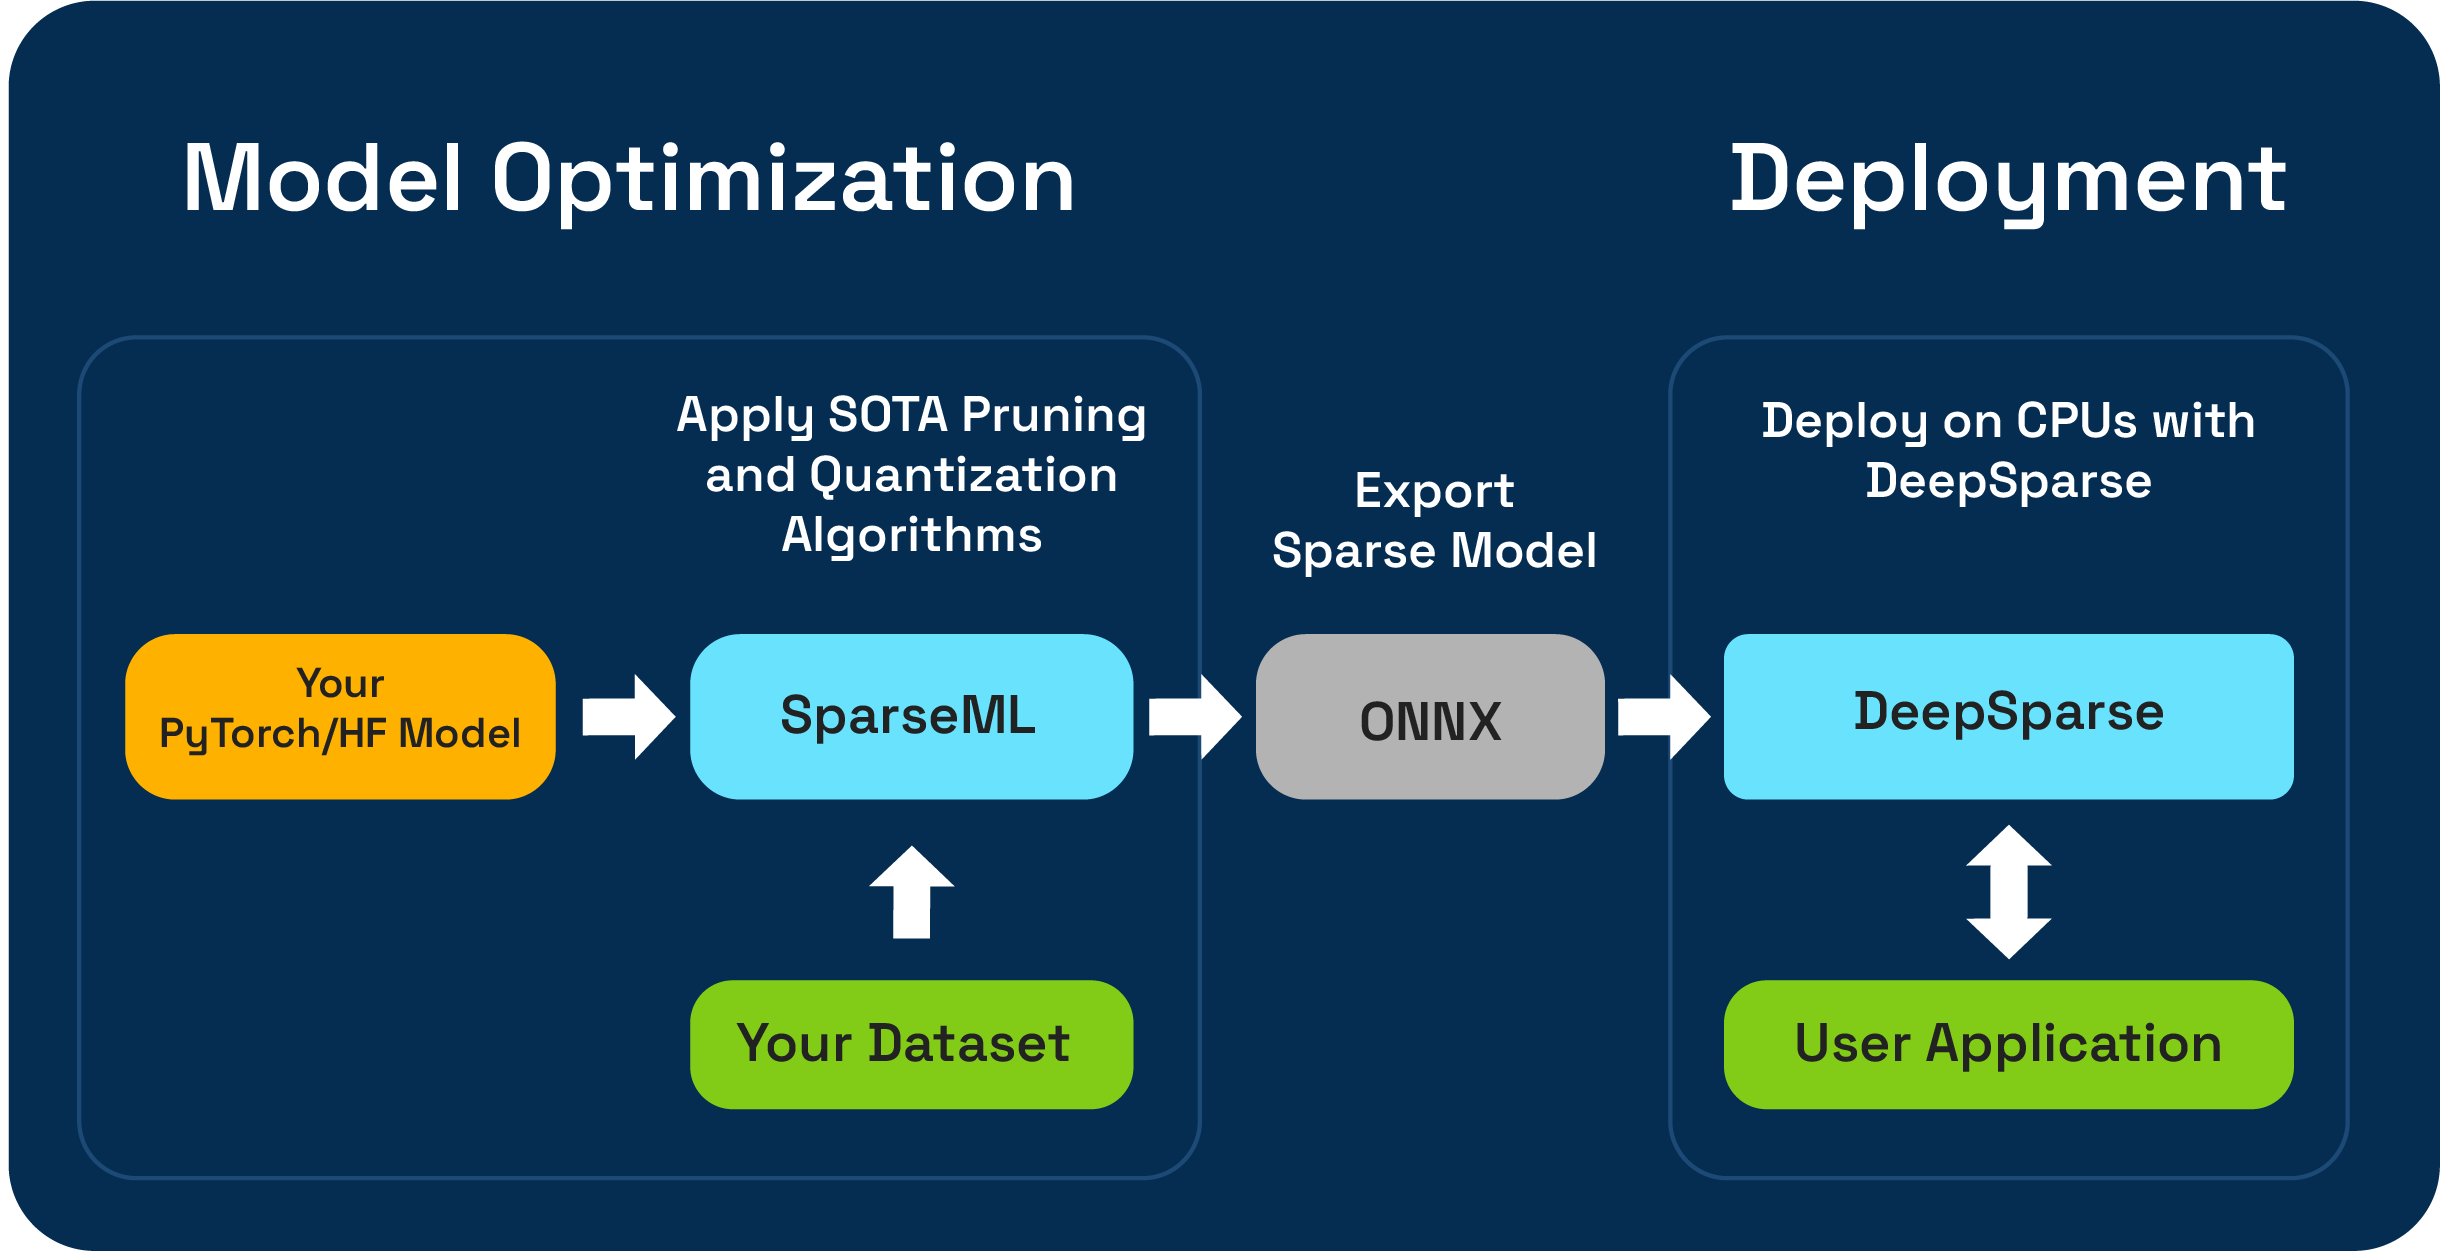
\includegraphics[width=\textwidth,height=5cm]{imgs/articles/sparseml-workflow.png}
    \caption{SparseML Pipeline \cite{sparseml}}
    \label{fig:sparseml}
  \end{minipage}
  \hfill
  \begin{minipage}[t]{0.49\textwidth}
      \centering
      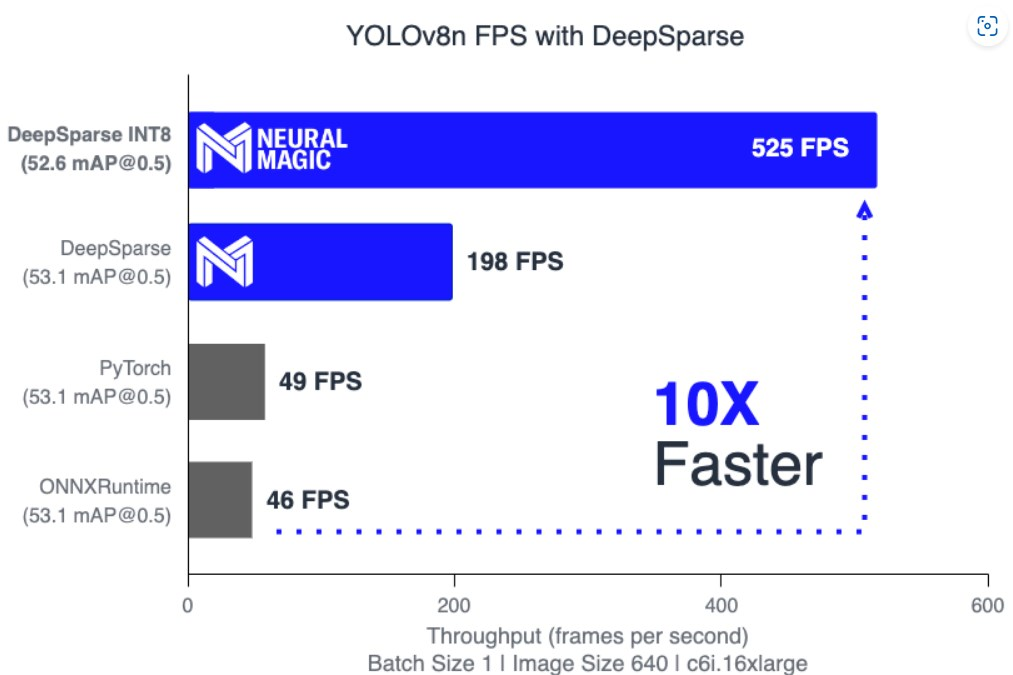
\includegraphics[width=\textwidth,height=5cm]{imgs/articles/yoloperf.jpg}
      \caption{DeepSparse Performance \cite{neuralmagic}}
      \label{fig:deepsparse}
      \end{minipage}
\end{figure}

However, efforts made by Neural Magic \cite{neuralmagic} in the optimisation of YOLOv5 and YOLOv8 show performance improvements of up to 10x on CPUs, through their open-source optimisation toolkit SparseML \cite{sparseml} and CPU inferencing runtime, DeepSparse \cite{deepsparse} as shown in \autoref{fig:sparseml} and \autoref{fig:deepsparse}. This is an incredibly promising result, as it shows that it is possible to run YOLOv8 in real-time on a CPU, which may help to achieve real-time inferencing on the Raspberry Pi 4, which is a key requirement of the project.

SparseML is a framework that helps automate the optimisation of deep learning models by employing sparsification techniques (the removal of unimportant weights from the model) and quantisation techniques (the reduction of the precision of the weights in the model) to reduce its computational complexity, and therefore its inference time. SparseML makes use of "recipes" to define the optimisation process, which can be customised to the specific requirements of the model, and can be used to optimise a range of different deep learning models, including YOLOv8. Pre-sparsified models exist on their "Model Zoo", which can be used to train models from scratch, or to fine-tune existing models.

DeepSparse is a CPU inferencing runtime that is designed to take sparsified models and run them on CPUs, with the aim of achieving real-time inferencing on CPUs. it is not neccessary to use DeepSparse with SparseML, as SparseML can be used to optimise models for any inferencing runtime, and DeepSparse can be used to run any model as long as it is in the correct format, typically the ONNX (Open Neural Network Exchange) format. This flexibility is very useful, as it allows for the use of the most appropriate inferencing runtime for the project.

\subsection{Training Methods}
When training a neural network, it is important to have training data. For a computer vision system, this means having a dataset of images that are representative of the conditions that the system will be used in and are well-labelled with bounding boxes and class labels. It is important to have a large dataset to ensure that the model is robust and generalises well, which is time-consuming to create.

To solve this problem, a paper by \citet{Yang_2023} proposes various training techniques, the most promising of which is semi-supervised learning. In this approach, the model is trained on a small labelled dataset, and then used to label a large unlabelled dataset, which is reviewed and corrected by a human.

This process is repeated until the model is sufficiently accurate, and then the model is trained on the large labelled dataset. This approach is very promising, as it allows for the training of a robust model with a large dataset, without the time-consuming process of manually labelling the entire dataset.

\subsection{Mechanical Design}
As the system is a mechatronic system, the mechanical design is a key component of the project. The mechanical design of the system must be able to transport components to the computer vision system, and then sort the components into designated bins. The mechanical design must be robust, reliable, and efficient and able to handle a range of different components. The mechanical design must also be able to interface with the other systems in the project, and so must be designed with this in mind. It is important to review existing sorting machines to inform the design of the project.
\subsubsection{Transport Mechanisms}
The paper by \citet{Dhenge2013MechanicalNS} depicts a conveyor belt system that transports nuts and bolts to a computer vision system for identification, which aligns with the goals of the project. The hardware prototype is shown in \autoref{fig:conveyor}, and a down-facing webcam is used to capture images of the components as they pass by. The webcam uses Principle Component Analysis (PCA) to identify the components, which will be discussed in the next section.

\begin{figure}[H]
  \hfill
  \begin{minipage}[t]{0.45\textwidth}
    \centering
    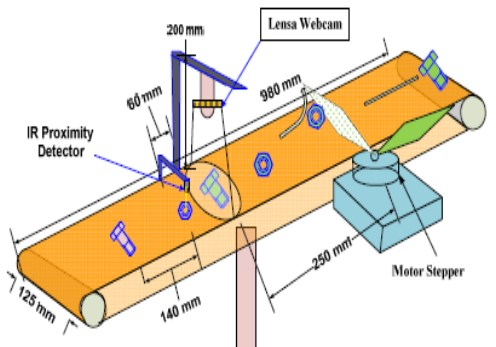
\includegraphics[width=\textwidth]{imgs/articles/conveyor.jpg}
    \caption{Nut and bolt sorter \cite{Dhenge2013MechanicalNS}}
    \label{fig:conveyor}
  \end{minipage}
  \hfill
  \begin{minipage}[t]{0.45\textwidth}
    \centering
    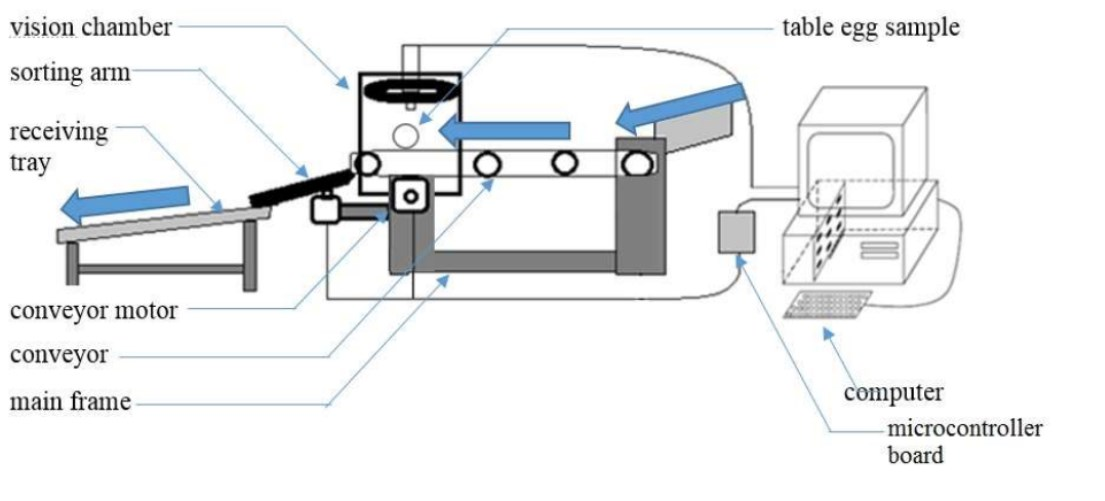
\includegraphics[width=\textwidth]{imgs/articles/eggsorter.jpg}
    \caption{Egg Sorter \cite{eggsorting}}
    \label{fig:eggsorter}
  \end{minipage}
  \hfill
\end{figure}

The components then separate into two chutes, one for nuts and one for bolts, using a stepper motor, which may be useful for the future design of the sorting system. Additionally, the approach taken by the paper \citet{eggsorting} to sort Philippine table eggs also features a similar conveyor belt system, a down-facing camera and an arm to sort the eggs into different categories as shown in \autoref{fig:eggsorter}. The approaches taken here are similar to industrial sorting systems seen in videos while researching for this project. This approach seems to answer three major design questions for the project; how to transport the components to the computer vision system; how to transport the components from the computer vision System to the sorting system; and the placement of the camera.

Other approaches include vibratory feeders \cite{s21217280}, which use precise vibrations to orientate and transport components, and pneumatic systems from \citet{ASEC2023-16267} (also suggested by project Supervisor Dr. Stott when dicussing transporting mechanisms in project meetings), use air pressure in tubes to transport components. These approaches require more complex hardware, and lack the easily achievable precision of the conveyor belt system, for example in the case of the pneumatic system, a complex network of tubes and valves and an air compressor is required, which is not practical for the project. Robotic arms are commonly used in the industry for sorting, however, this is not viable as this would either require an expensive robotic arm, or a complex system of motors and actuators to move the components.

From the approaches above, it seems that a conveyor belt with a down-facing camera is the most viable approach to transporting the components.

% Initially, the aim was for the system to be semi-autonomous, with a design allowing the camera to face upwards. This configuration would enable the user to place the component on an acrylic plate directly above the camera for immediate identification, enabling easy user interaction as the view of the component is not obstructed. Having the camera face-down would block the user's view of the component, which would be an inconvenience, and as such, the current design of the system features an up-facing camera. However, this will be changed to reflect the research outlined above, in the next stage of the project.

\subsubsection{Bowl Feeders}
While researching for this project, and especially in videos \cite{videobowlfeeder}, it seems most industrial sorting machines use a Vibratory Bowl Feeder (VBF) to help feed components into the sorting system.

\begin{figure}[H]
  \hfill
  \begin{minipage}[t]{\textwidth}
    \centering
    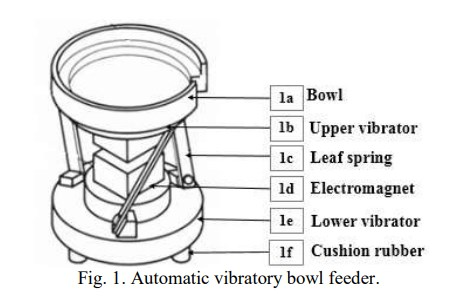
\includegraphics[height=8cm]{imgs/articles/feeder.jpg}
    \caption{VBF \cite{nam2019design}}
    \label{fig:feeder}
  \end{minipage}
\end{figure}

As shown in \autoref{fig:feeder}, the VBF consists of a bowl that vibrates coupled with a spring and electromagnet. The paper by \citet{nam2019design} explores the optimal design of a VBF for USB keycaps, by attempting to identify the ideal parameters for the structure of the bowl, sorting track, mounting adapter, and suspension system. The paper also uses modal analysis to determine the natural frequencies of the system and uses this to avoid resonant conditions that might cause inefficient or erratic operation.

This paper is useful as it provides a comprehensive overview of the design of a VBF, and provides a good starting point for the design of the VBF. In the future, the project may make use of one for fully autonomous sorting. The paper also provides a good overview of the design considerations for the VBF, and so can be used as a reference during the design process.

Additionally, \citet{REINHART2010191} delve into a mathematical model of a VBF, optimising more on the overall performance of the VBF rather than efficiency, and \citet{ForceAnalysisofVibratoryBowlFeeder} provides a good overview of the forces involved in the operation of a VBF, strengthening the basis for its design and viability. The paper by \citet{zhang2019design} outlines a sorting system for vials and does not make use of a VBF, instead opting for a turntable design that mechanically orientates the vials. It primarily operates
by using a design that is specific to the geometry of the vials, and so does not apply to this project, however, it does provide a good insight into the design of a sorting system.

An alternative to the VBF could be a robotic arm; fine control over movement would be necessary as the components are small and may be tangled, however, as mentioned before would require its own set of sensors and camera systems. As the components can be tangled, there are not many viable alternatives to the VBF or a robotic arm, so between these two solutions, it seems that the VBF is the most viable approach if the system is to be fully autonomous, as the vibrations of the VBF would help to untangle the components.

\subsection{Commerical Systems}
\todo{complete this section with a few youtube videos}
\subsection{Key Takeaways}
After reviewing the literature, the following key takeaways were made:

The most viable approach to the problem of component identification is to use a CNN, specifically the YOLOv8 architecture, as they are very effective at classification tasks, which translates to being able to identify electronic components. With the ability
to optimise the model using SparseML and DeepSparse, the model may be able to run on the Raspberry Pi 4 in real-time, which is a key requirement of the project.

The most viable approach to the problem of component transportation seems to be a conveyor belt system with a down-facing camera, and so the design of the mechatronics and the computer vision system will be based on the research outlined above.

A VBF is the most viable approach to the feeding mechanism of the sorting system, and so the design of the VBF (if employed in the project) will be based on the research outlined above.

Additionally, the YOLOv8 architecture will be employed, making use of the SparseML and DeepSparse optimisation tools with semi-supervised learning to train the model.
